\section{Travail réalisé}
\label{sec:work}
  \subsection{Reconstruction de CFG}
    \subsubsection{Définitions}
      \paragraph{Instructions et fichier exécutable}
      { Les instructions machine, ou simplement instructions, sont les
        opérations codées en langage machine qu'offre un processeur.

        Un fichier exécutable contient l'ensemble des instructions d'un
        programme écrit dans un langage de haut niveau (ou en assembleur) qui a
        été compilé (ou respectivement assemblé) pour une plateforme
        particulière. }
  
      \paragraph{Bloc de base et graphe de flot de contrôle}
      { Un bloc de base est une séquence d'instructions qui n'a qu'un point
        d'entrée, sa première instruction, et qu'un point de sortie, sa dernière
        instruction.

        Le graphe de flot de contrôle d'un programme est un graphe orienté dans
        lequel les n{\oe}uds représentent les blocs de base issus du programme
        et les transitions représentent les enchainements possibles entre les
        différents blocs de base lors de l'exécution du programme.
    
        De manière formelle, un CFG est un tuple $(V, E, i)$, où les n{\oe}uds
        $V$ correspondent aux blocs de bases, les transitions $E \subset V
        \times V$ sont les chemins du flots de contrôle et $i \in V$ représente
        le n{\oe}ud de départ, c'est à dire le n{\oe}ud qui n'a pas de
        transition entrante. }

    \subsubsection{Méthodes de reconstruction}

      % Utilisation d'un analyseur sémantique de fichiers exécutables pour la
      % reconstruction de CFG.

      Le fichier exécutable à analyser est en amont soumis à une analyse
      sémantique réalisée par l'outil \textsc{HARMLESS}~\cite{KBB12}. Cette
      analyse séquentielle des instructions du fichier exécutable produit un
      fichier de données textuelles associant à chaque instruction un ensemble
      d'informations la caractérisant. Parmi ces informations on peut citer par
      exemple : l'adresse mémoire de l'instruction, une representation textuelle
      de l'instruction issue de son désassemblage, ou encore les registres
      utilisés en lecture et en écriture par l'instruciton. Ce fichier de
      données est l'unique entrée de l'outil décrit ici.

      \medskip

      Cet outil\footnote{\texttt{https://github.com/LiberH/tool}} est écrit en
      Haskell~\cite{Mar10}. Il réalise de manière préliminaire une analyse
      syntaxique du ficher d'entrée pour en manipuler le contenu via une
      strucutre de données appropriée. Cette structure représente la liste
      ordonnée des instructions du programme.
      
      \begin{figure}
        \centering
        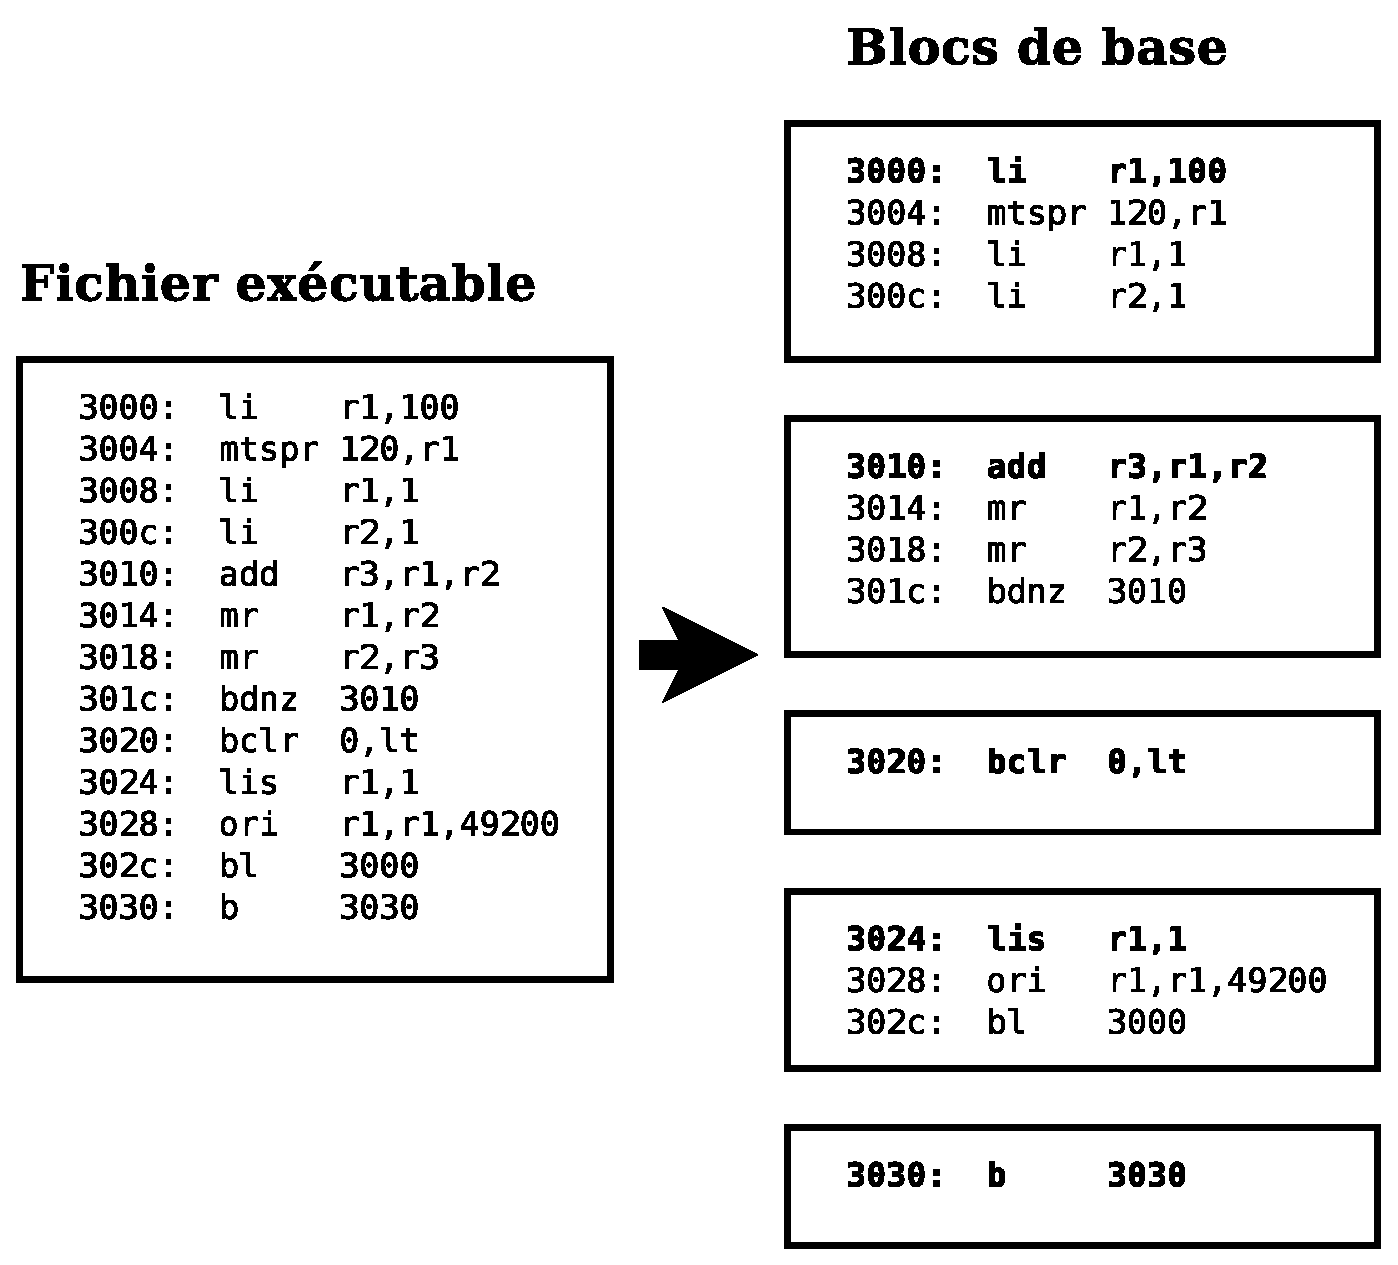
\includegraphics[scale=0.3]{recons1.eps}
        \caption{Processus de reconstruction de blocs de base}
        \label{fig:recons1}
      \end{figure}

      \paragraph{Reconstruction des blocs de base}
      { La prémière étape nécessaire à la reconstruction du CFG consite en la
        reconstitution des blocs de base du programme.

        Pour ce faire, il est tout d'abord nécessaire d'identifier les points
        d'entrée de blocs de base. Une instruction est une entrée de bloc de base
        si elle se trouve être :
        \begin{itemize}
          \item le point d'entrée du programme ;
          \item une cible de saut ;
          \item immédiatement après une instruction de saut ;
          \item la première instruction du fichier exécutable.
        \end{itemize}

        Les blocs de base sont construits en parcourant séquentiellement la
        liste ordonnée des instructions du programme et par accumulation des
        instructions se trouvant entre un point d'entrée de bloc de base inclus
        jusqu'au suivant exclus. La figure \ref{fig:recons1} donne un exemple
        d'un telle reconstruction. }

      \begin{figure}
        \centering
        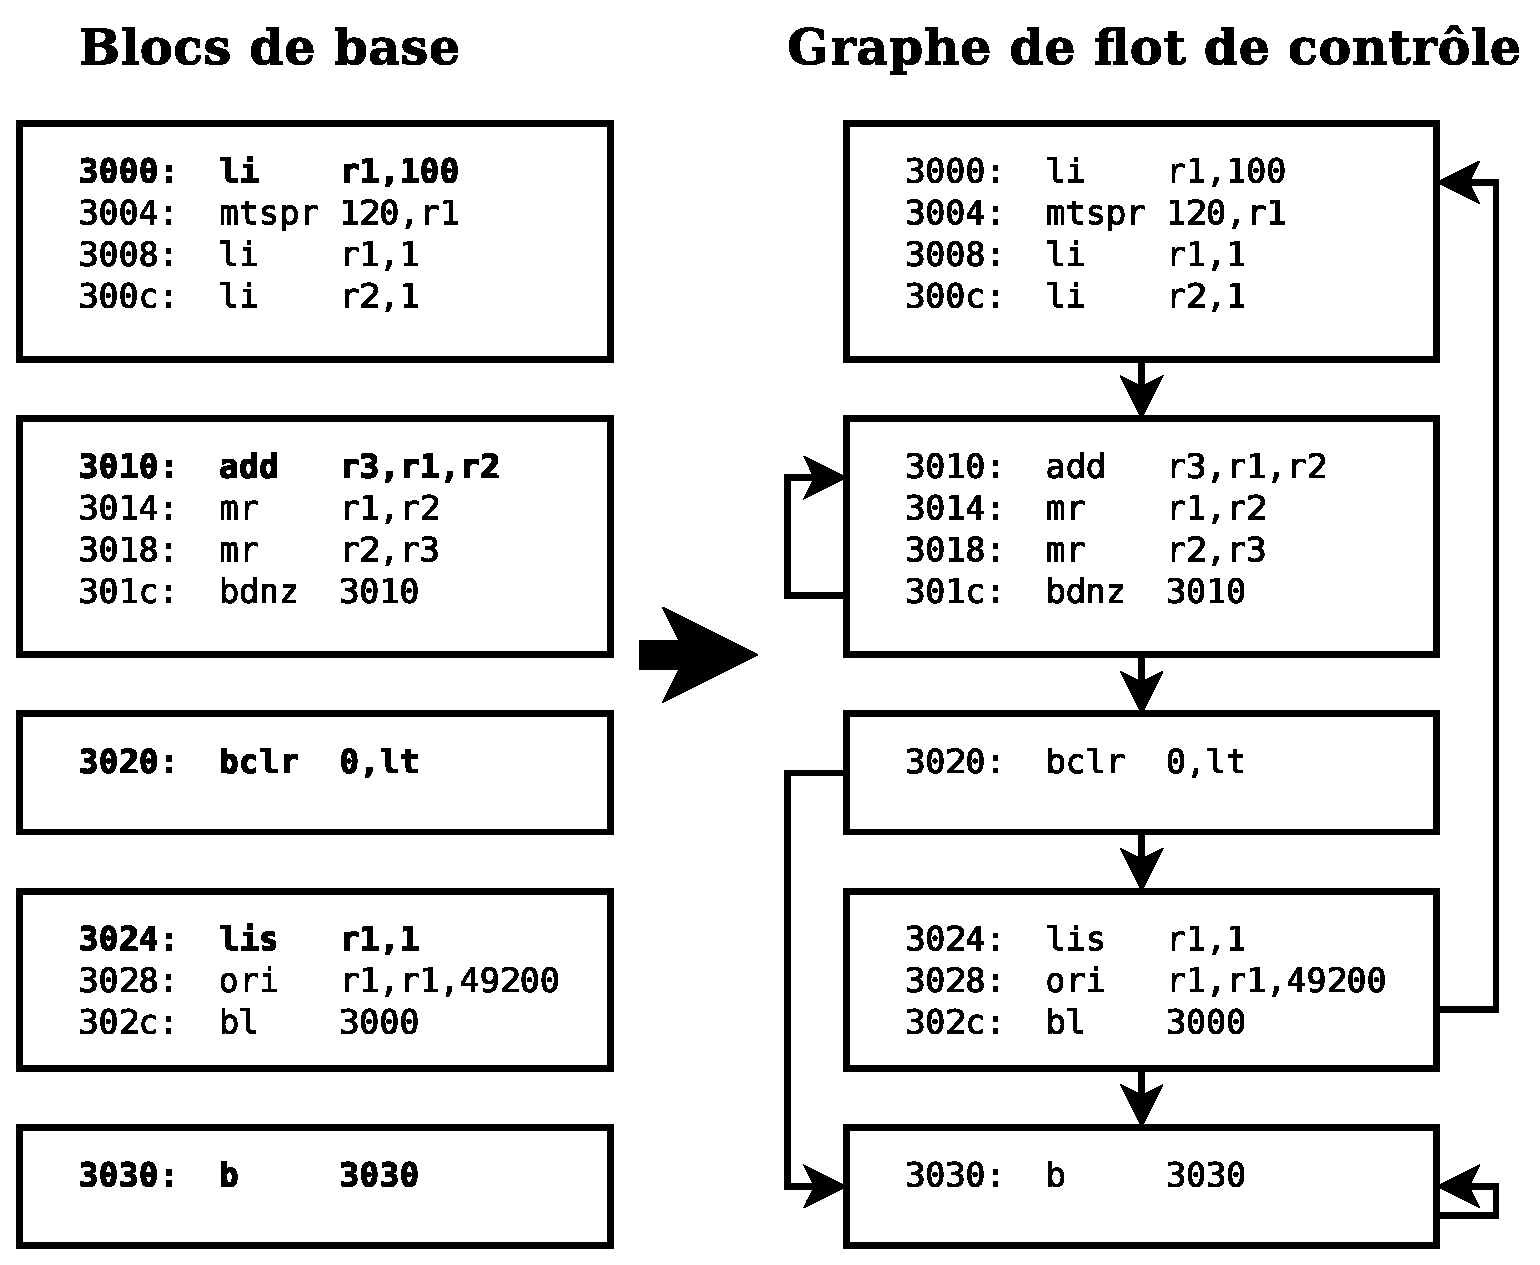
\includegraphics[scale=0.3]{recons2.eps}
        \caption{Processus de reconstruction d'un CFG}
        \label{fig:recons2}
      \end{figure}

      \paragraph{Reconstruction de CFG}
      { % Utilisation d'une bibliothèque d'analyse et de transformation de CFG
        % pour le slicing de CFG.

        Afin de procéder à la reconstruction du CFG en elle-même l'outil fait
        usage de \textsc{Hoopl}, une bibliothèque de manipulation de CFG en
        Haskell~\cite{RDP10}. Cette bibliothèque permet de définir simplement
        des analyses de flots de données ainsi que des transformations sur les
        CFG manipulés.

        \medskip
        
        Il est tout d'abord nécessaire d'identifier les n{\oe}uds. C'est une
        tâche triviale vis-à-vis de la définition d'un CFG. Il faut également
        identifier le n{\oe}ud de départ. C'est le n{\oe}ud correspondant au
        bloc de base issu du point d'entrée du programme.

        Il faut ensuite contruire les transitions. Elles sont obtenues
        itérativement en associant à chaque bloc de base les cibles possibles de
        son point de sortie. La figure \ref{fig:recons2} donne un exemple d'un
        telle reconstruction.

        Cette tâche est difficile dans le cas de sauts indirects. Lorsqu'il est
        impossible de déterminer les cibles possibles du point de sortie d'un
        bloc de base il est fait usage d'un n{\oe}ud \textit{inconnu}. Ces
        cibles seront par la suite déterminées par le \textit{slicing} du CFG. }
        

  %% TODO:
  %\subsection{Slicing de CFG}
